
This tutorial aims to generate a molecule in which two halfs of a PAMAM dendrimer are connected by a Poly-ethylenegycol (PEG) linker.
Similarly to the PAMAM/PPI-Half tutorial, this tutorial needs to use both modules in order to prepare the molecule conveniently (Figure \ref{fig:PAMAMPEG}).

\begin{figure}
    \centering
    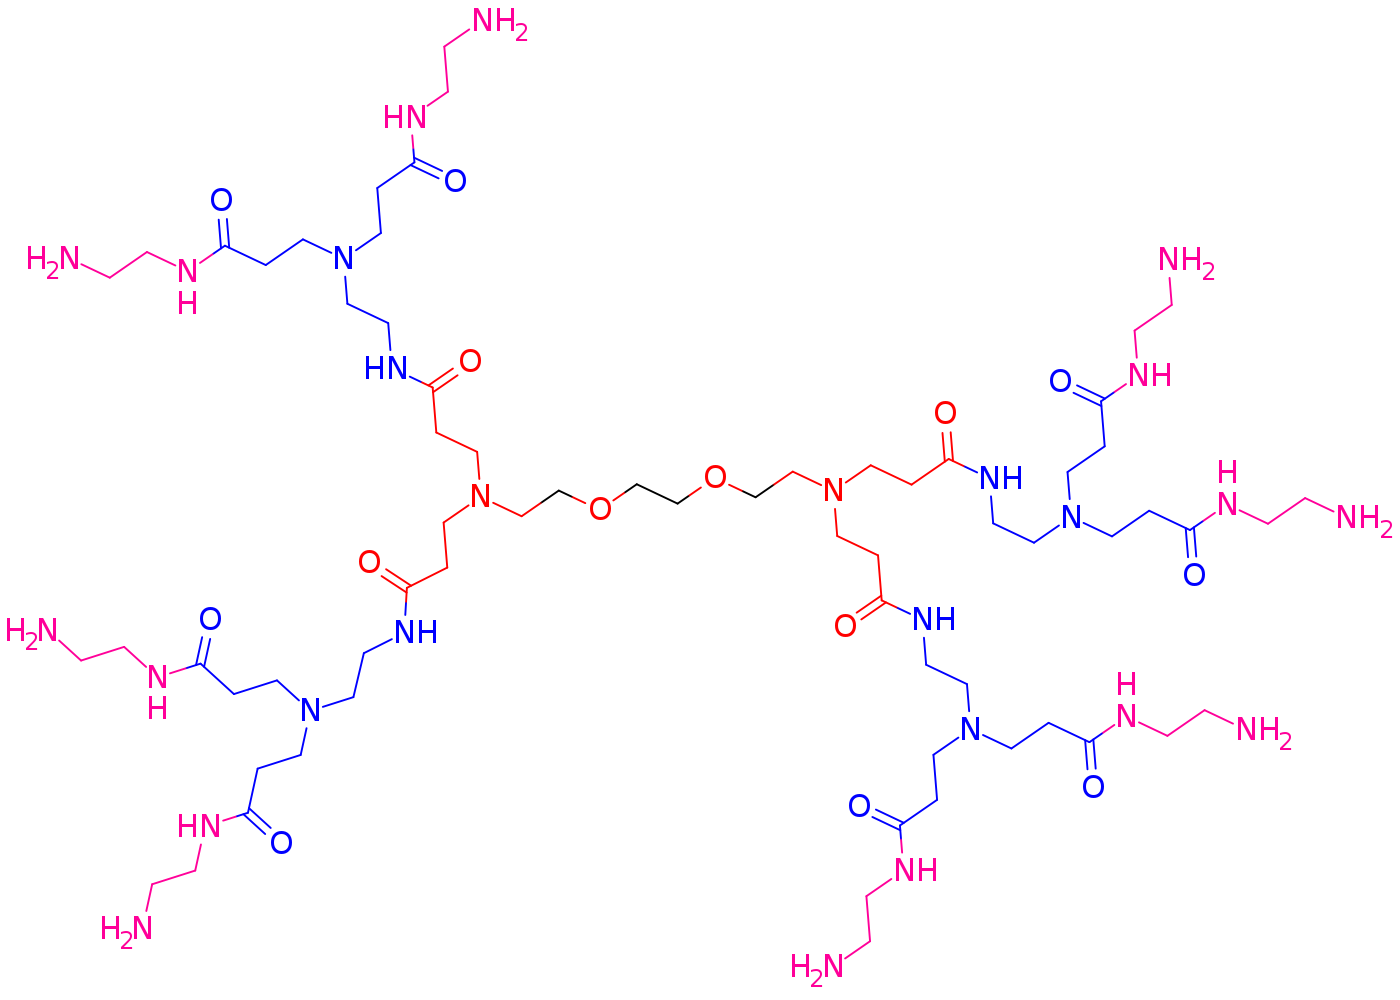
\includegraphics[width=0.5\textwidth]{PAMAM_PEG/PAMAMPEG.png}
    \caption{PAMAM-PEG dendrimer in which each side is connected by a PEG polymer. The PAMAM core block is illustrated in red, intermediary and core blocks are displayed in blue and pink, respectively. The PEG moiety of the molecule is placed between the two PAMAM halfs.}
    \label{fig:PAMAMPEG}
\end{figure}

All needed files are provided in demo directory:

\begin{lstlisting}
<path/to/pypolybuilder>/demo/gromacs_format/polymer/PAMAM_PolyEtyleneglycol
\end{lstlisting}
\dirtree{%
.1 PAMAM\_PolyEtyleneglycol.
.2 coreHalf\_PAMAM.itp.
.2 inter\_PAMAM.itp.
.2 ter\_PAMAM.itp.
.2 ethyleneglycol.itp.
.2 list\_param.itp.
.2 connect.in.
.2 run.
.3 PAMAM\_PEG.sh.
.3 PAMAM\_PEG.top.
.3 mdp.
}

All the following procedure for building the PAMAM dendrimer, in which its core is split into two halfs connected by a PEG polymer, is automated in the available bash script \texttt{how\_to\_run\_this\_example.txt}.

For building this molecule, we will make the dendritic part of the molecule first and then connect two of these, using the network module to get all BBs together.
The core BB for the dendrimer module is a PAMAM core split in the middle.
Intermediary and terminal blocks are the same as used in PAMAM tutorial (See Figure \ref{fig:PAMAMPEGBBs}).

\begin{figure}
    \centering
    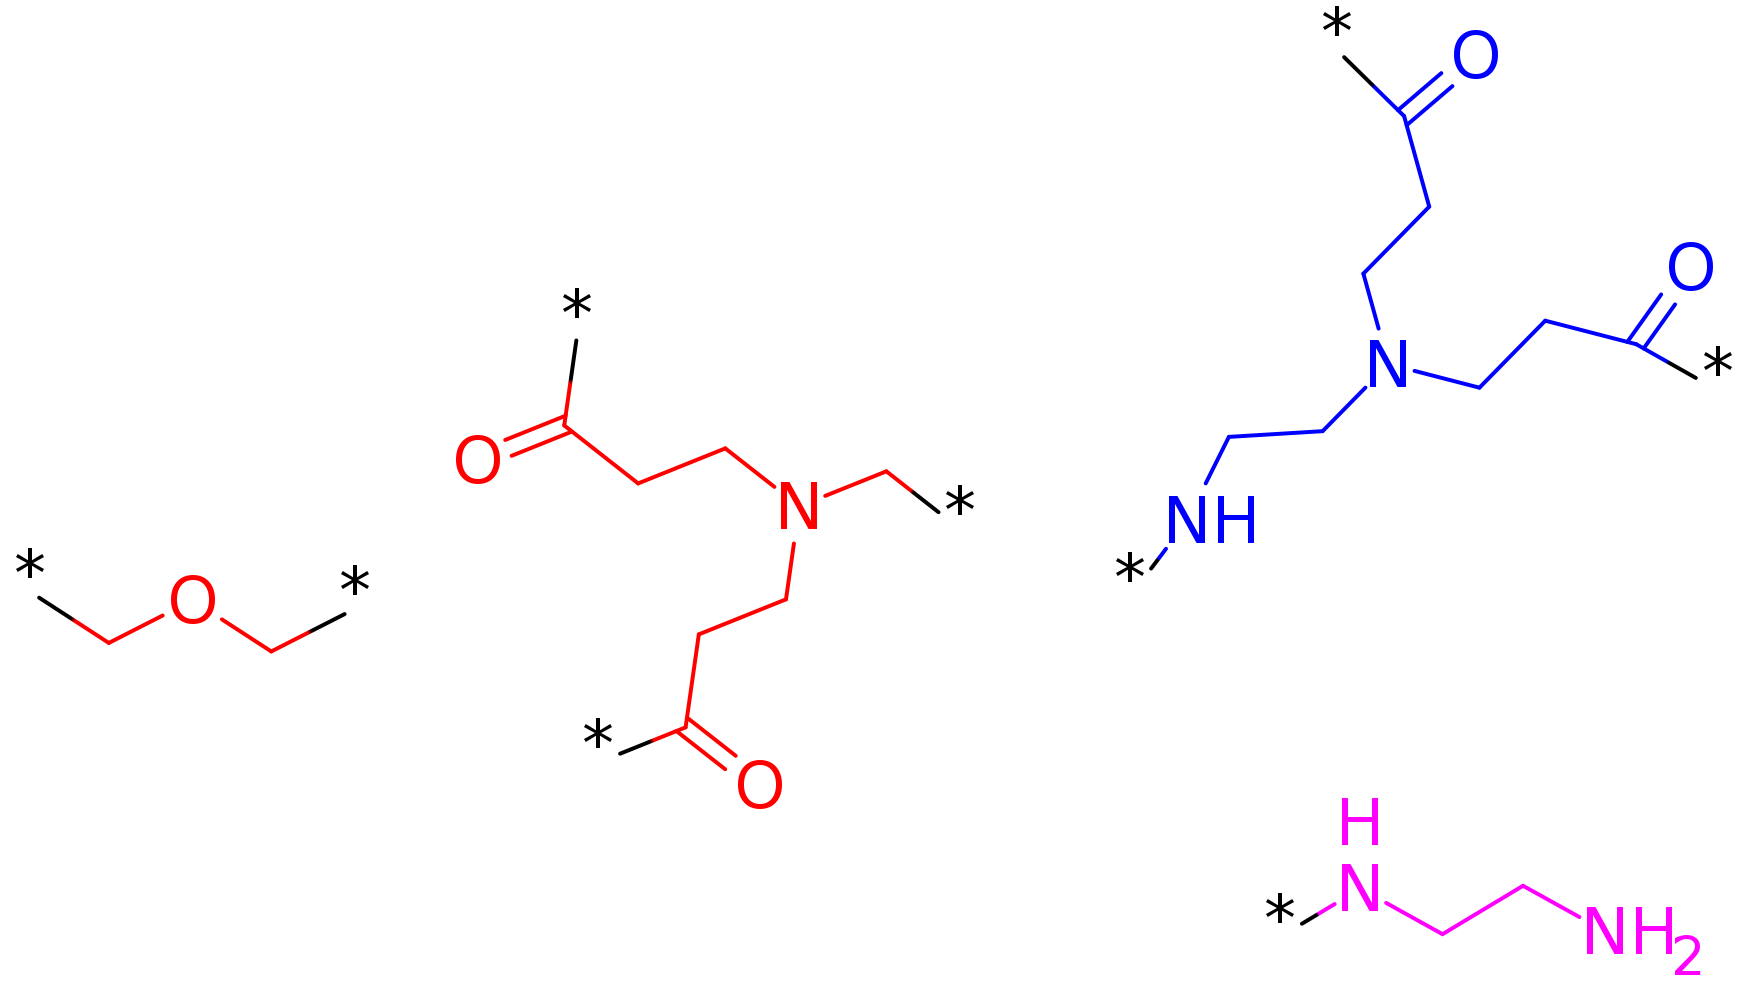
\includegraphics[width=0.6\textwidth]{PAMAM_PEG/PAMAMPEGBBs.png}
    \caption{PAMAM-PEG dendrimer BBs. The PAMAM core, intermediary and terminal blocks are displayed in red, blue and pink, respectively. The PEG monomer is placed on the left of the figure.}
    \label{fig:PAMAMPEGBBs}
\end{figure}

The dendrimer module can be called to generate the dentritic part of the molecule by using the following command line to build the first part of the molecule using PAMAM BBs:

\begin{lstlisting}
python3 ../../../../__main__.py \
--core=coreHalf_PAMAM.itp \
--inter=inter_PAMAM.itp \
--ter=ter_PAMAM.itp \
--params=list_param.itp \
--ngen=1 \
--name=PAMH \
--output=PAMAMhalf.itp \
--nogeom \
--dendrimer
\end{lstlisting}

Here the usage of dendrimer module is exactly the same as when generating a whole dendrimer.
However, the \texttt{[ branches ]} field is made in a way that pyPolyBuilder uses only the two available branching points.

\begin{lstlisting}
[ branches ]
;  donor   acceptor
    0      6
    0      9
\end{lstlisting}

In the first pyPolyBuilder call, the option \texttt{--nogeom} was used because we are not interested in optimizing the geometry of a molecule, which is only an intermediate step of building the final MTF.
Hence, this options can be used to save time skipping the optimization stage and the generation of a coordinates file for the intermediary molecules.

\begin{figure}
    \centering
    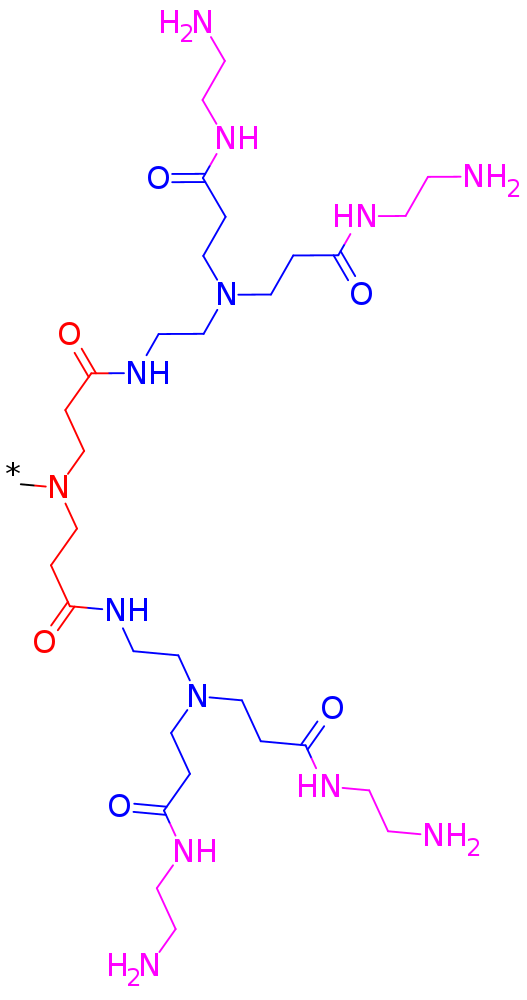
\includegraphics[width=0.3\textwidth]{PAMAM_PEG/PAMAMPEGHalf.png}
    \caption{PAMAM part of the PAMAM-PEG dendrimer. The color scheme is adopted in accordance with the Figure \ref{fig:PAMAMPEGBBs}.}
    \label{fig:PAMAMPEGHalf}
\end{figure}

Once we have built the dendritic part of the molecule (Figure \ref{fig:PAMAMPEGHalf}), the network module can be called to connect every BB we need.
For instance, we will use the blocks in Figure \ref{fig:PAMAMPEGBBs} to build the molecule in Figure \ref{fig:PAMAMPEG}.
In order to do that, the \texttt{connect.in} file defines how the BBs are connected.
To make it simple, only two monomers of PEG will be used.

\begin{lstlisting}
#[ BUILDING BLOCKS ]
1   PAMH
2   EG
3   EG
4   PAMH

#[ CONNECTS ]
1    2    1    1
2    3    3    1
3    4    3    1

\end{lstlisting}

After building all the BBs, the final molecule will be done and can be visualized in any software (Figure \ref{fig:PAMAMPEGHalf}).
The command line to gather all BBs together is the following one:

\begin{lstlisting}
python3 ../../../../__main__.py \
--bbs=PAMAMhalf.itp,etyleneglycol.itp \
--in=connect.in --params=list_param.itp \
--name=PAMPEG --output=PAMAM_PEG.itp \
--gro=PAMAM_PEG.gro \
--network
\end{lstlisting}

Once this last command line is done, the dendrimer will be completed, including its geometry optimized in vacuum (Figure \ref{fig:PAMAMPEGPPB}).
It is strongly suggested that the geometry generated by pyPolyBuilder be energy-minimized in a simulation package.
The procedure of energy minimization, equilibration, and simulation, is automated in a script file called \texttt{PAMAM\_PEG.sh} in the run directory.

\begin{figure}
    \centering
    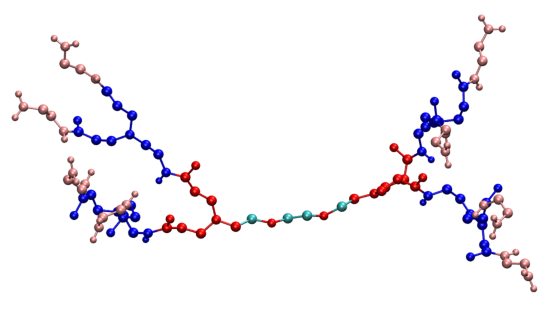
\includegraphics[width=0.5\textwidth]{PAMAM_PEG/PAMAM_PEG_PPB.pdf}
    \caption{PAMAM\_PEG dendrimer in which each side is connected by a PEG linker. The PAMAM core block is illustrated in red, intermediary and core blocks are displayed in blue and pink, respectively. The PEG moiety of the molecule is placed between the two PAMAM halfs.}
    \label{fig:PAMAMPEGPPB}
\end{figure}

The outputs from pyPolyBuilder \texttt{PAMAM\_PEG.*} needs to be copied to the run directory and the input path for the gromacs package in the \texttt{PAMAM\_PEG.sh} needs to be changed.
\texttt{PAMAM\_PEG.sh} can be run in order to automatically solvate the molecule, minimize the energy of the system, equilibrate it for 100 ps in nvt and npt ensembles, and carry out 100 ps of molecular dynamics simulation.
Figure \ref{fig:PAMAMPEGSOL} shows a snapshot of an equilibrated conformation of the PAMAM-PEG molecule.

\begin{figure}
    \centering
    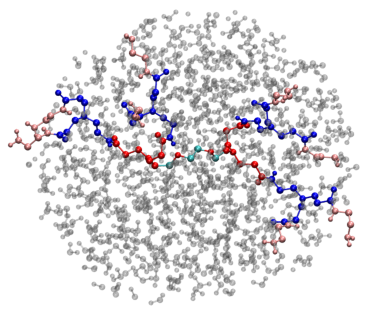
\includegraphics[width=0.5\textwidth]{PAMAM_PEG/PAMAM_PEG_SOL.pdf}
    \caption{PAMAM\_PEG dendrimer in water. The color scheme is in accordance with Figure \ref{fig:PAMAMPEGPPB}. The water molecules are displayed as translucent silver molecules.}.
    \label{fig:PAMAMPEGSOL}
\end{figure}